\chapter{Implementation}\label{ch:implementation}
% Fall: what was built, with the key design choices. Spring adds the AI parts.

This chapter describes the system as it stands on 20 November 2026: a backend with 216 automated
tests and a web client with 39, built in pull requests up to \#100. Everything described here runs
without an AI model; the applicant enters the fields. Reading the fields with a model is being
added (Section~\ref{sec:ai-design}).

\section{Development environment and tools}\label{sec:tools}
The backend is written in Python 3.12 with FastAPI, Pydantic and SQLAlchemy 2, and stores its
data in PostgreSQL 17 with the pgvector extension, started with Docker Compose. Database changes
are Alembic migrations (six so far). Dependencies are managed with uv and pinned in a lock file.
The web client uses React 19, TypeScript, Vite, Tailwind CSS and TanStack Query; its tests run
with Vitest and Testing Library.

Every change follows the same path: an issue with a completion criterion, a branch, a pull
request, a green run of GitHub Actions, and a squash merge. The \texttt{main} branch is protected
and requires two checks: lint and tests of the backend against a PostgreSQL service, and type
check, tests and build of the web client. Decisions are recorded as architecture decision records
in \texttt{docs/decisions/}.

An AI assistant was used to draft code, tests and documentation; Section~\ref{sec:ai-use}
describes how it was used and how its output was checked.

\section{Backend}
The service is created by an application factory and grouped by concern: checklist, accounts,
application files, documents, checks and destinations. Settings come from environment variables;
the API does not start without a database address and a document key, because neither has a safe
default. Two health endpoints separate \emph{the process is up} from \emph{the database can be
reached}.

\paragraph{Accounts and sessions (ADR 0004).} Users register with an e-mail address and a password
that is hashed with Argon2id. A session is a random token; the browser holds it in a cookie that
scripts cannot read, and the database stores only its SHA-256, so a copy of the database does not
give access. Requests that change state must carry a custom header, which a form on another site
cannot add. Five failed logins within fifteen minutes block further attempts for that address.

\paragraph{Application files.} A file belongs to one user and one trip and records the requirement
set that was active when it was created. Every query is limited to the owner; a file of another
user is answered with \emph{not found}, not with \emph{forbidden}, so its existence is not
revealed. Each change of step is stored as a dated event.

\paragraph{Documents (ADR 0005).} Upload is refused until the user has accepted the current
version of the consent text. The type of a file is read from its first bytes, not from its name;
PDF, JPEG and PNG up to 10\,MB are accepted. Location data is removed from photographs. Each
document is then encrypted with its own AES-256-GCM key, and that key is itself encrypted with a
master key kept outside the repository (Figure~\ref{fig:envelope}). The file is stored under a
random name; its original name, which often contains the applicant's name, is encrypted too.
Deleting a document removes the row and the file together, and documents expire thirty days after
the trip.

\begin{figure}[ht]
  \centering
  \small
  \begin{tabular}{@{}ccccc@{}}
    master key & $\rightarrow$ & data key & $\rightarrow$ & file, file name, \\
    (\texttt{.env}) & wraps & (one per document) & encrypts & field values \\
  \end{tabular}
  \caption{Envelope encryption of a document. The document identifier is bound to every
  encrypted value, so a value cannot be moved to another document.}
  \label{fig:envelope}
\end{figure}

\section{Requirement data and source snapshots}
The requirements live in YAML files, not in code (Chapter~\ref{ch:design},
Listing~\ref{lst:rule}). A loader validates them and cross-checks them: every requirement and rule
must cite a known source, every field a rule reads must exist with the right type, and no rule may
read a document that no checklist item asks for. A seed command loads the files into the database
as a \emph{requirement set} whose identifier is the SHA-256 of the files. Loading unchanged files
does nothing; changed files give a new set, and older sets are kept, so a check made earlier can
still show the rules it used.

A snapshot command fetches every official source, stores the content only when its hash differs
from the last one, and appends every attempt to a manifest. It was run on 23 October, 5, 10 and
23 November 2026 (the run of the week of 17 November was missed): 21 page snapshots, of which 7
had a new hash; none of them changed a requirement (Section~\ref{sec:design-sources}).

\section{Field entry and rule engine}\label{sec:engine}
For every uploaded document the applicant enters the fields its type defines; the two fields about
language are asked only where a translation rule of the destination reads them. Values are
validated against the field type and stored encrypted with the document's key.

The rule engine is a set of pure functions: it receives the rules, the documents with their
values, and the trip, and returns one result per rule. It reads neither the database nor the
clock. Every date is compared with the trip or with the application date of the file, so a check
gives the same result whenever it is run, and each rule kind of Table~\ref{tab:rule-kinds} can be
tested with invented documents. A rule ends in one of four states:

\begin{description}[style=nextline,leftmargin=2.2cm]
  \item[passed] the entered values satisfy the rule;
  \item[failed] an entered value breaks it;
  \item[incomplete] a value the rule needs has not been entered, or cannot be compared;
  \item[skipped] the document the rule reads is not uploaded; the missing document is reported
    instead.
\end{description}

Separating \emph{incomplete} from \emph{failed} matters to the applicant: an empty field is a
task, not a problem with the application. Each issue names the document, the field, the value
found and the value expected, which is what \reqid{FR-10} asks for. Names are compared without
case, Turkish letters, punctuation or order, so that the name in the passport and the name printed
on a booking in capital letters with the surname first are recognised as the same.

Where a source does not state a limit that a check needs, the engine uses an assumption that is
marked as such in the code and recorded in ADR 0006: a bank statement must end at most one month
before the application, the newest payslip must be from the application month or the two before,
and an amount in another currency than the rule's is not compared. Chapter~\ref{ch:evaluation}
returns to them as threats to validity.

A check can be kept. A kept check stores the state of every rule and where each issue is, but not
the compared values, because those are personal data that stay encrypted with their documents;
the page shows current values by running the check again.

\section{Web client}\label{sec:web}
The client is one responsive application in Turkish and English; all interface text comes from
two translation files, and a test fails when their keys differ. It talks to the API on its own
origin, so the session cookie stays first-party.

The checklist page needs no account: the visitor chooses a destination and a profile and sees the
documents and rules, each with the official passage and a link. A second public page lists, per
destination, where and when to apply, fingerprints and fees, again with the source of each fact.
After logging in, a three-step wizard creates an application file. The application page
(Figure~\ref{fig:app-page}) shows the route, the days to the appointment, a readiness ring with
one segment per document and the dated steps; below it come the document table with the upload
panel and the rules with their states (Figure~\ref{fig:app-rules}). A findings page (Figure~\ref{fig:app-findings}) groups the result into missing documents, problems,
rules with missing details and passed rules, each problem with the passage of its source, and
lists the kept checks with the change since the previous one. The figures show the demo file of
an employed applicant to the Netherlands with one labelled error applied: the guest name on the
hotel booking differs from the name in the passport.

\begin{figure}[ht]
  \centering
  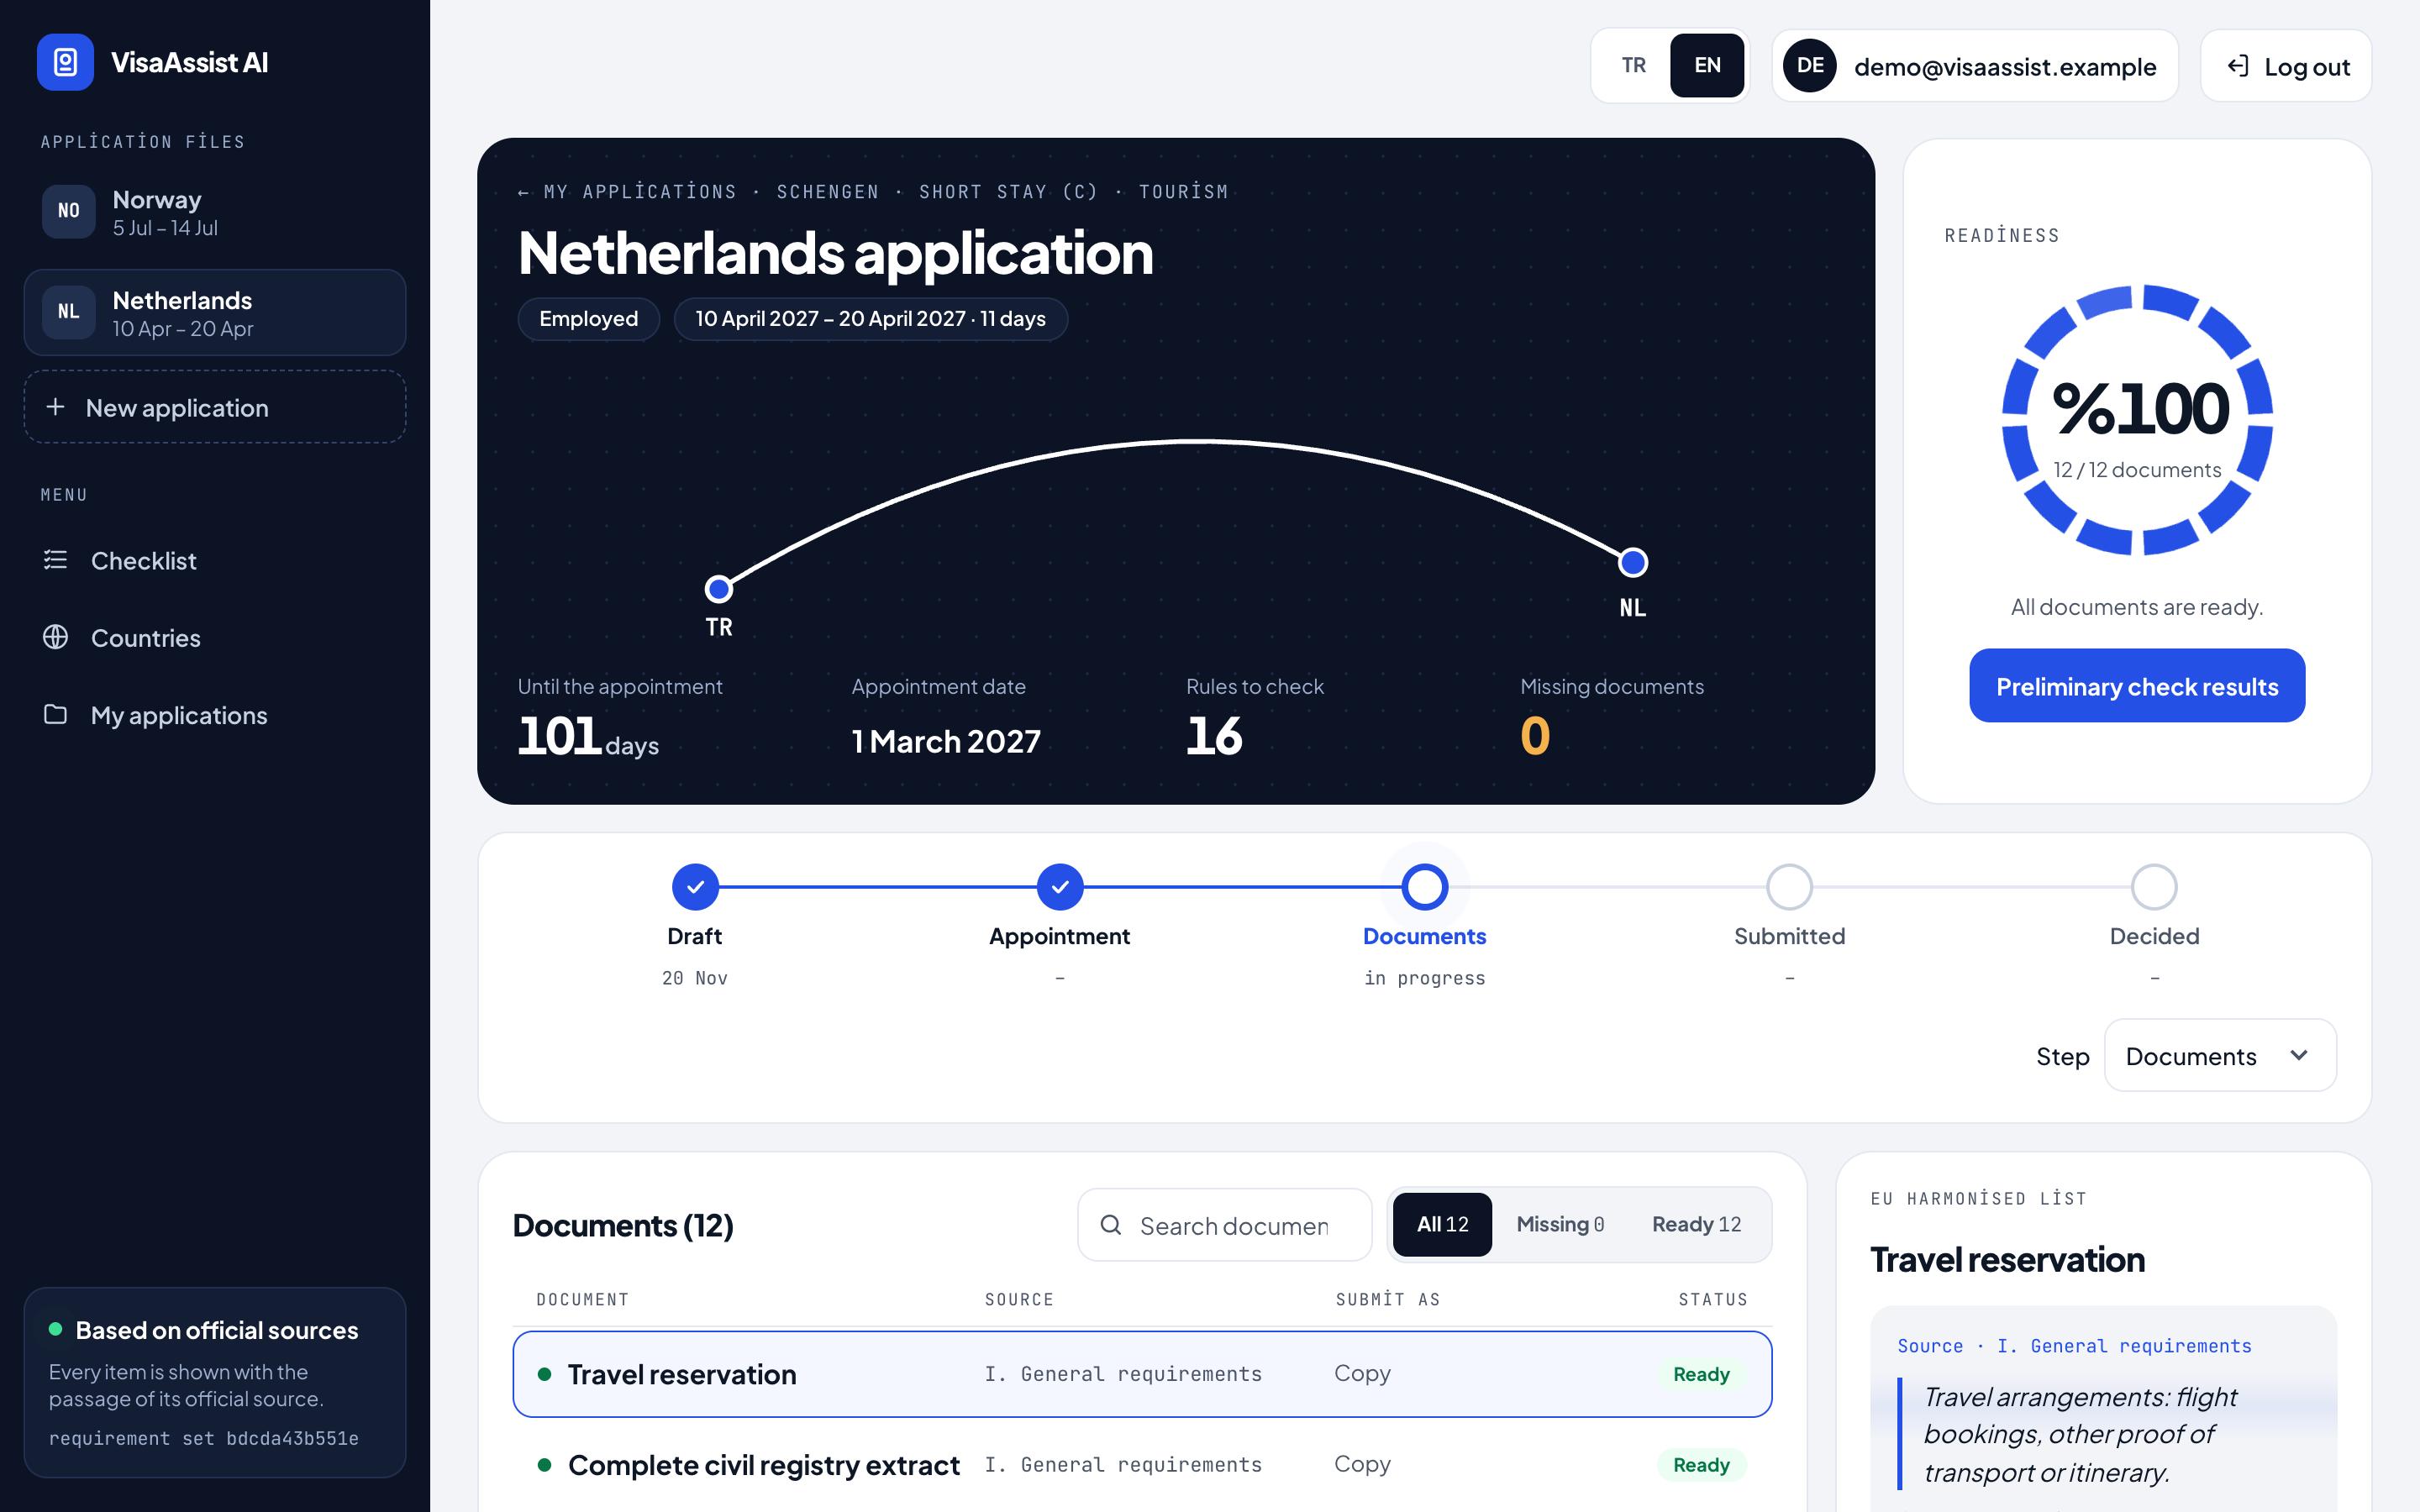
\includegraphics[width=\textwidth]{shot-application.png}
  \caption{Application page of the running system with the demo file for the Netherlands: route,
    days to the appointment, readiness ring and steps.}
  \label{fig:app-page}
\end{figure}

\begin{figure}[ht]
  \centering
  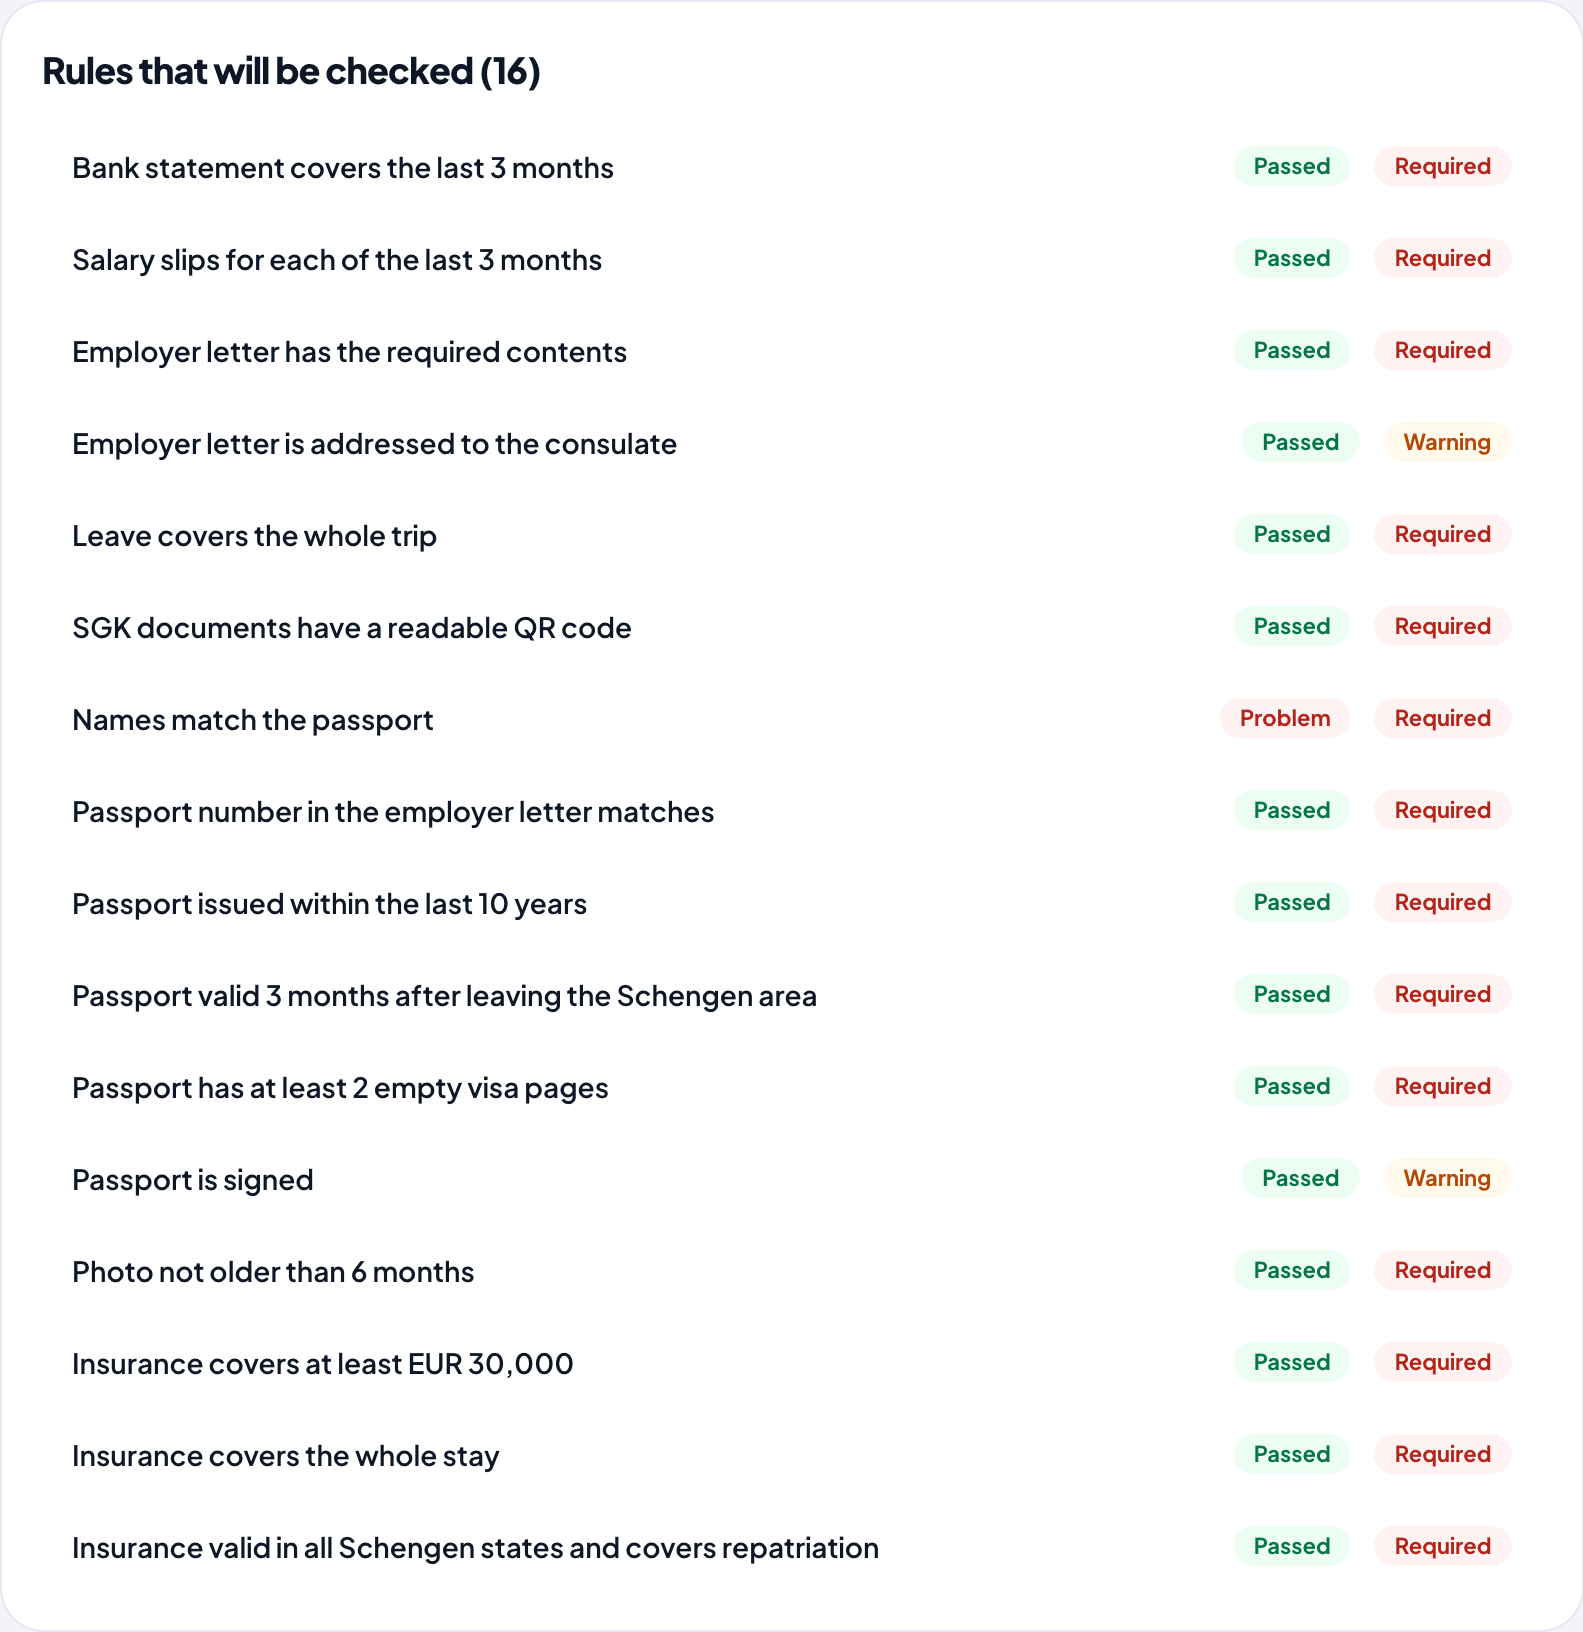
\includegraphics[width=\textwidth,height=0.75\textheight,keepaspectratio]{shot-rules.png}
  \caption{Rules of the same file with the state of the preliminary check; the name rule reports
    a problem.}
  \label{fig:app-rules}
\end{figure}

\begin{figure}[ht]
  \centering
  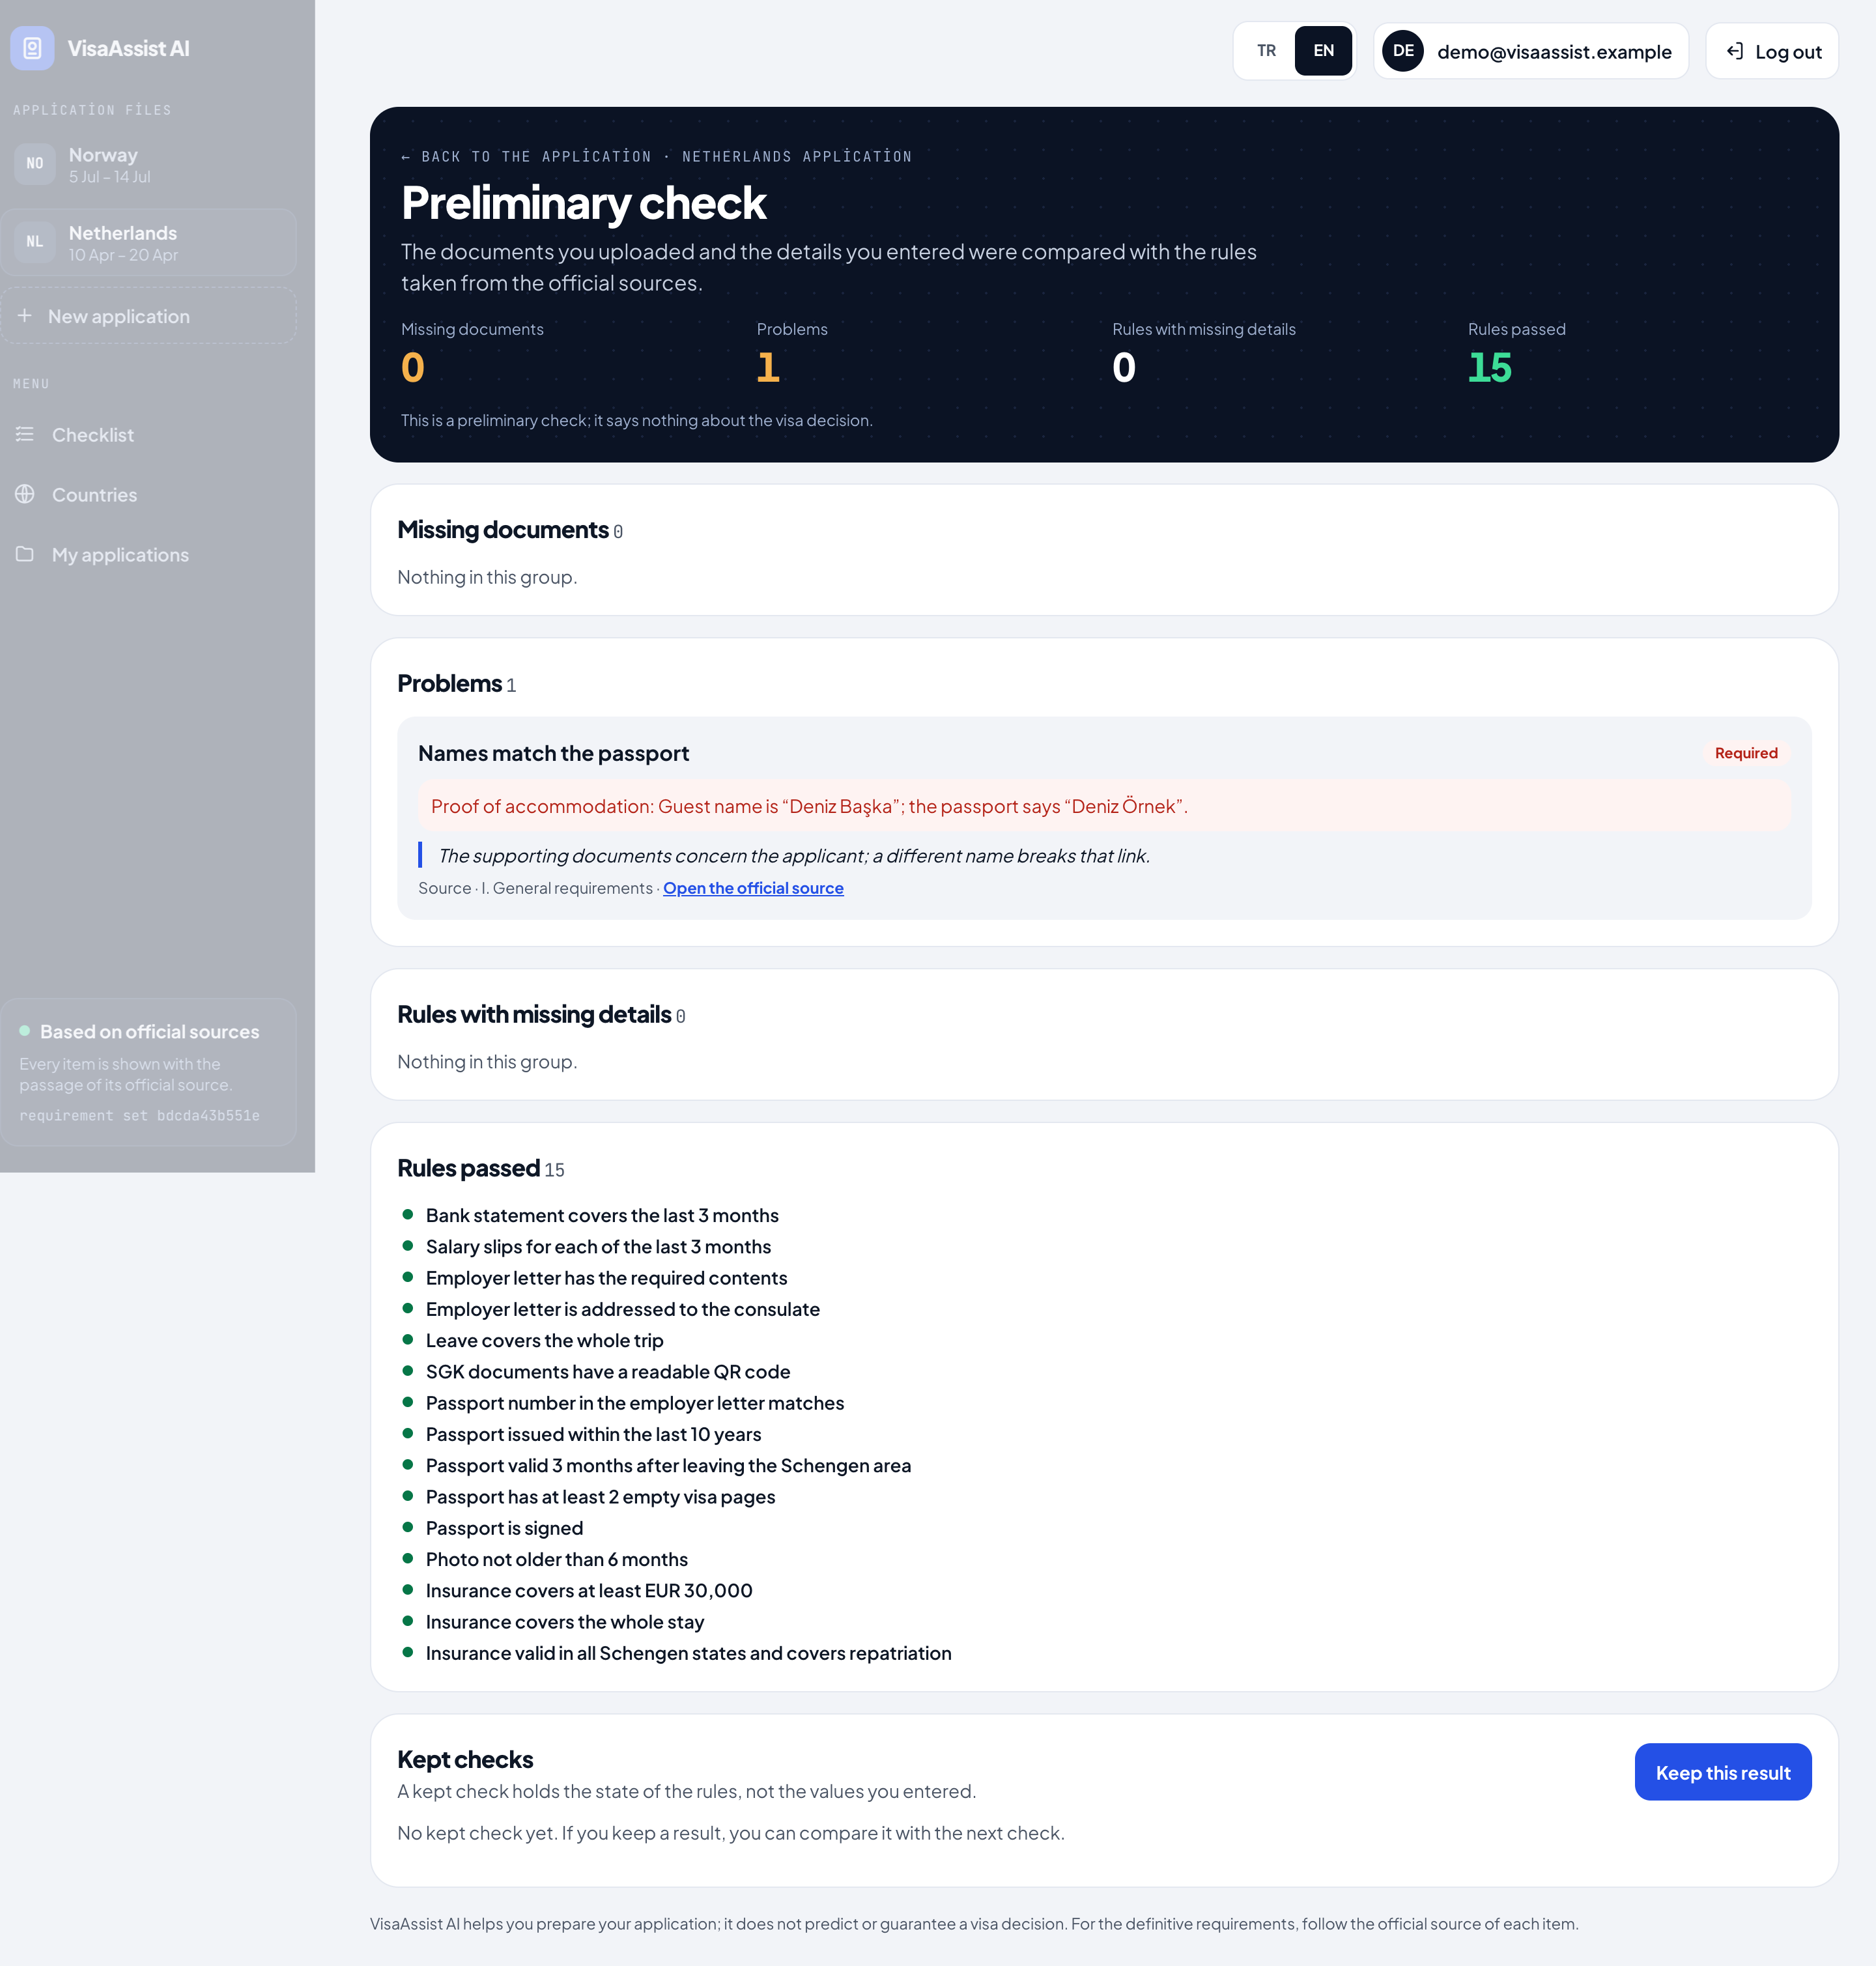
\includegraphics[width=\textwidth,height=0.8\textheight,keepaspectratio]{shot-findings.png}
  \caption{Findings page: the problem names the documents, the field and the official passage.}
  \label{fig:app-findings}
\end{figure}

The flow was tried on a phone, including a photograph taken with the camera. Three layout
problems were found and corrected: date fields wider than their card, the page zooming when a
field was focused, and a document table whose status column needed a sideways scroll.

\section{Demo files and setup}\label{sec:demo}
Two synthetic application files serve the demonstration and the evaluation of
Chapter~\ref{ch:evaluation}: an employed applicant to the Netherlands with 14 documents and a
student to Norway with 9. Every person, number and organisation in them is invented, and their
titles say SAMPLE. Each file holds field values that satisfy every rule of its destination and
profile, and a list of labelled errors; an error changes one thing, either removing a document or
setting one value, and names the finding it must produce. A loader checks every value against the
field types of the catalogue, so a demo file cannot drift from the data model.

A second command loads the files into the running system as a demo account: one application file
per demo file, a one-page PDF marked SAMPLE for every document, and the field values entered as an
applicant would enter them. Labelled errors can be applied on request, so the findings page has
something to show. Because the command replaces the account's files, it accepts only addresses
under a reserved example domain.

The whole system starts with one command, \texttt{docker compose --profile app up --build}: the
database, the API, which updates the tables and loads the requirement data and the demo account
when it starts, and the web client served by nginx, which forwards \texttt{/api} to the API on
the same origin. Only the web client's port is published, and only on the local machine
(\reqid{NFR-07}).

\section{State against the plan}
The roadmap placed this work in weeks 9 to 13 of the fall semester. All of it was finished by
20 November, in week 9: the demo files and the one-command setup, the last two items of the fall
plan, were completed in that week. The time gained goes to the change decided on 20 November:
reading the fields with a model and comparing the model with and without the rule engine
(Section~\ref{sec:ai-design}). The administrator's pages and the remaining AI components belong
to spring.
